\begin{figure}
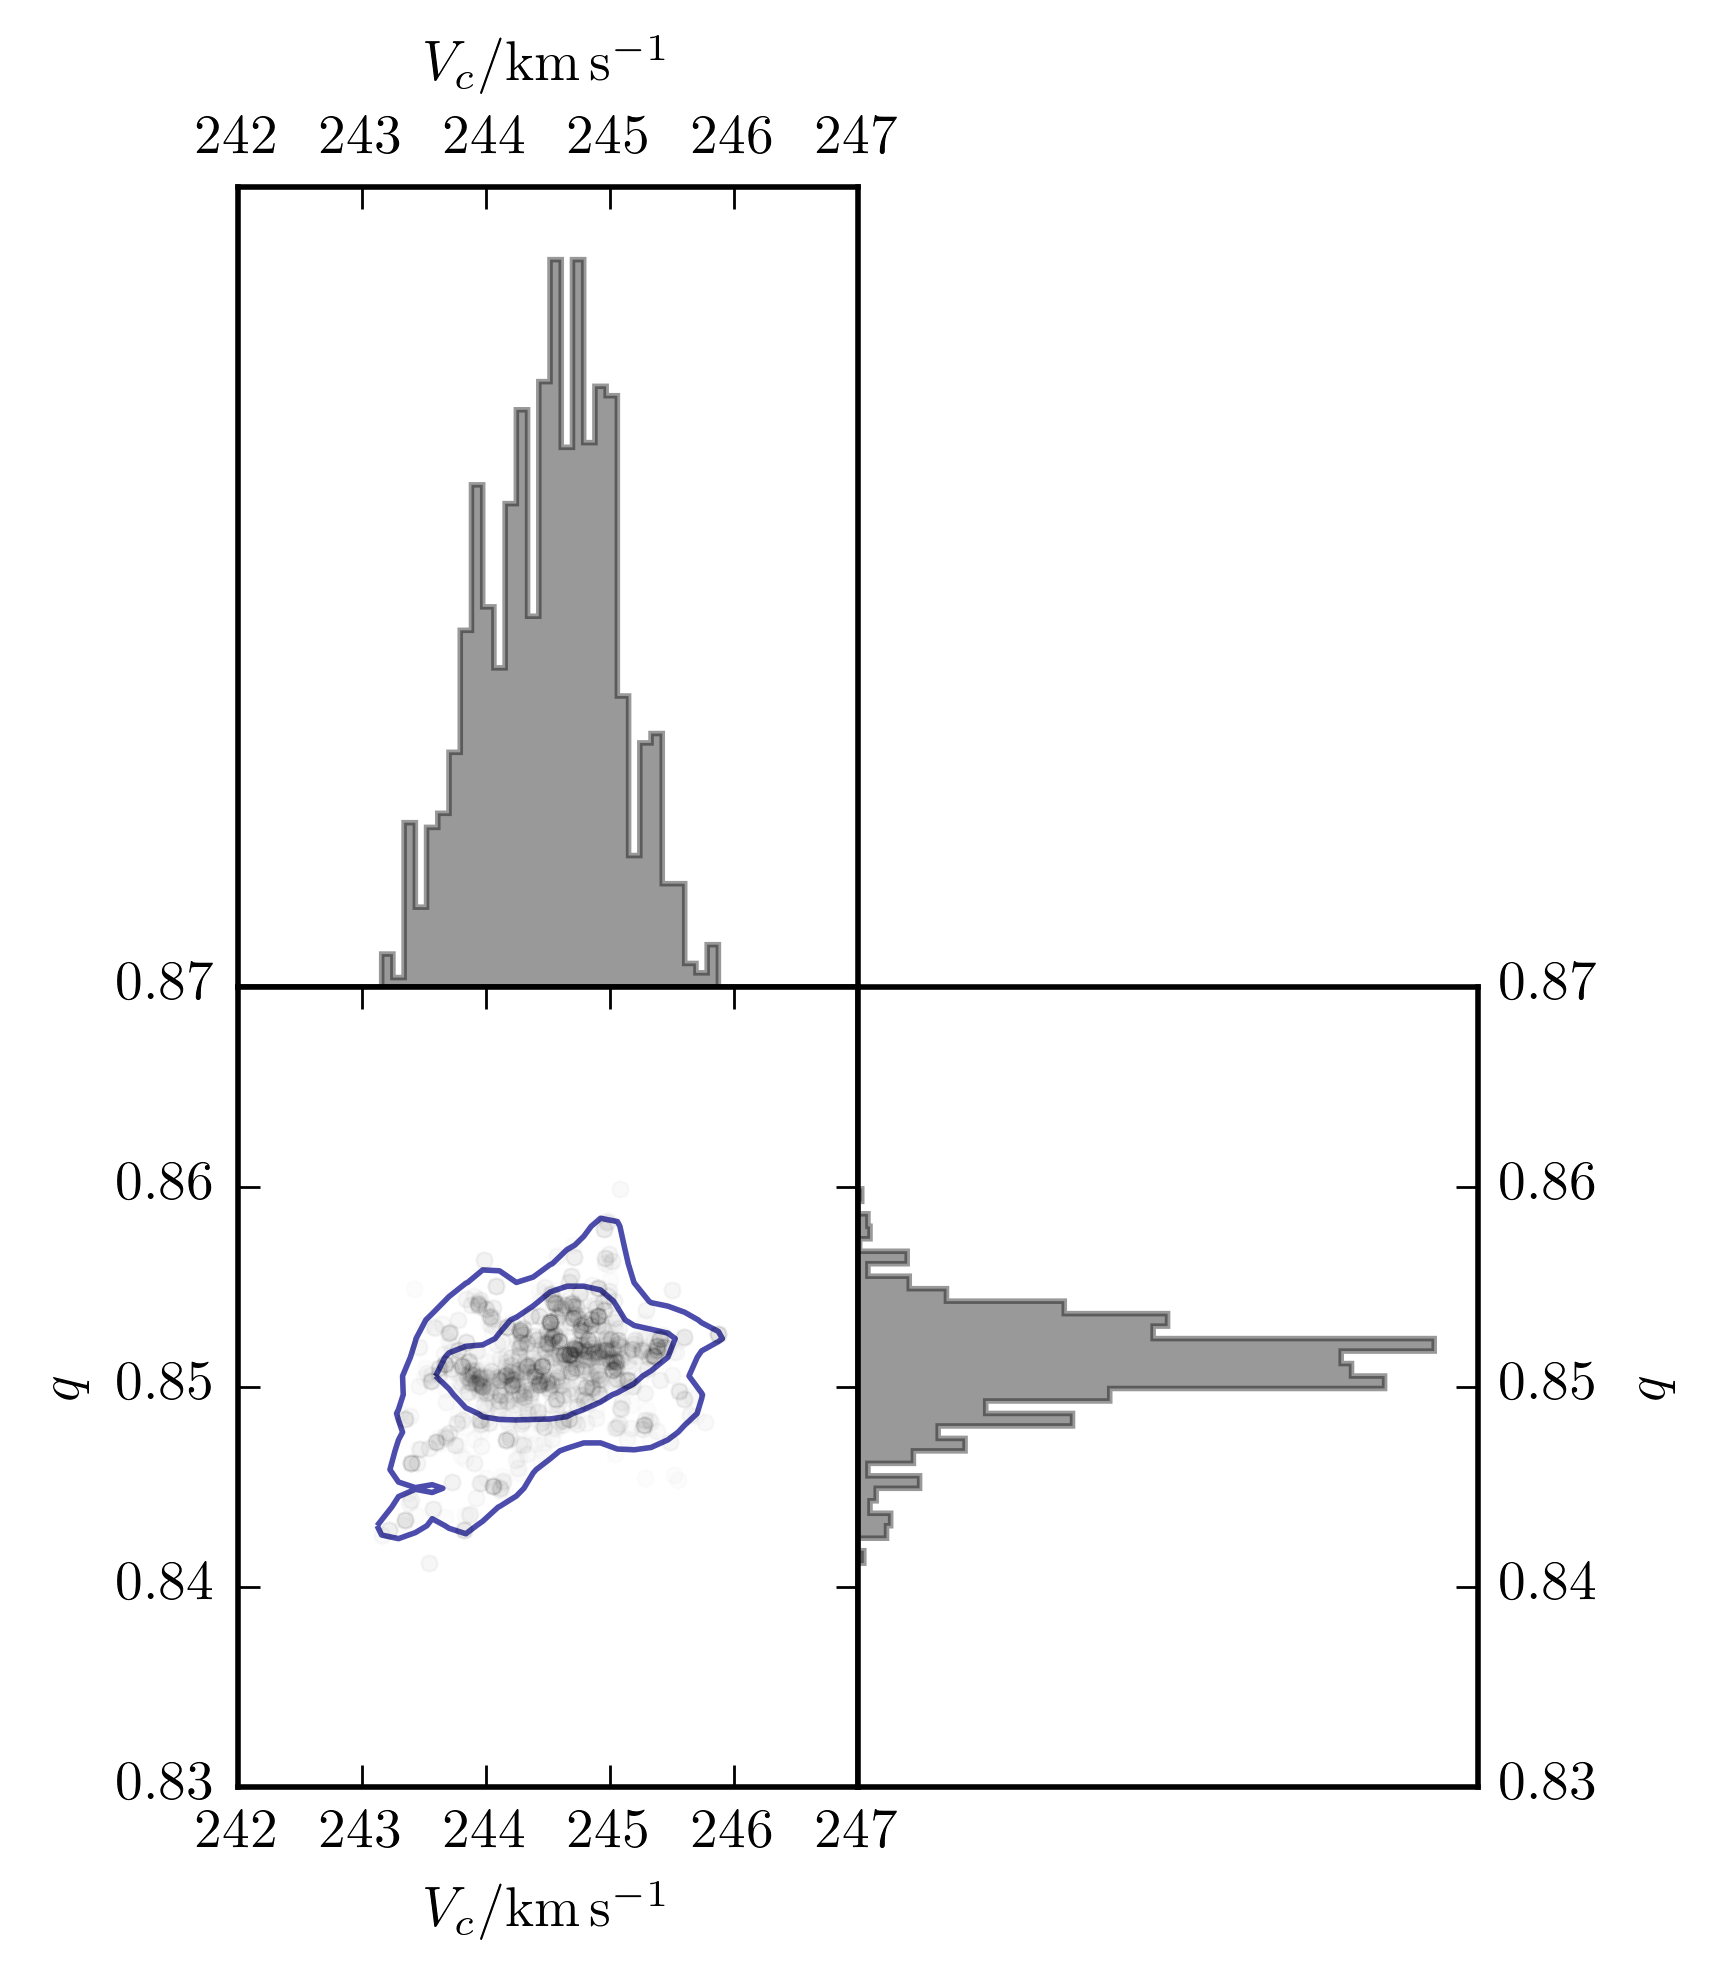
\includegraphics[width=83mm]{./figures/jason_results_logarithmic.png}
  \caption{Jason's results (Sec.~\ref{ssec:jason_results})}
  \label{plot_jason_results_logarithmic}
\end{figure}

\begin{figure}
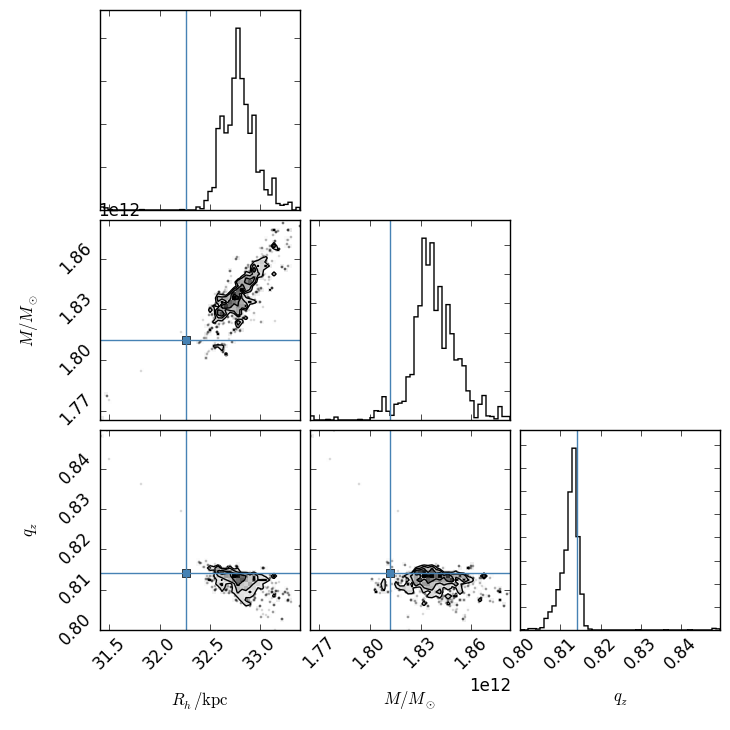
\includegraphics[width=83mm]{./figures/jason_results_truepot.png}
  \caption{Jason's results (Sec.~\ref{ssec:jason_results})}
  \label{plot_jason_results_truepot}
\end{figure}

\begin{figure}
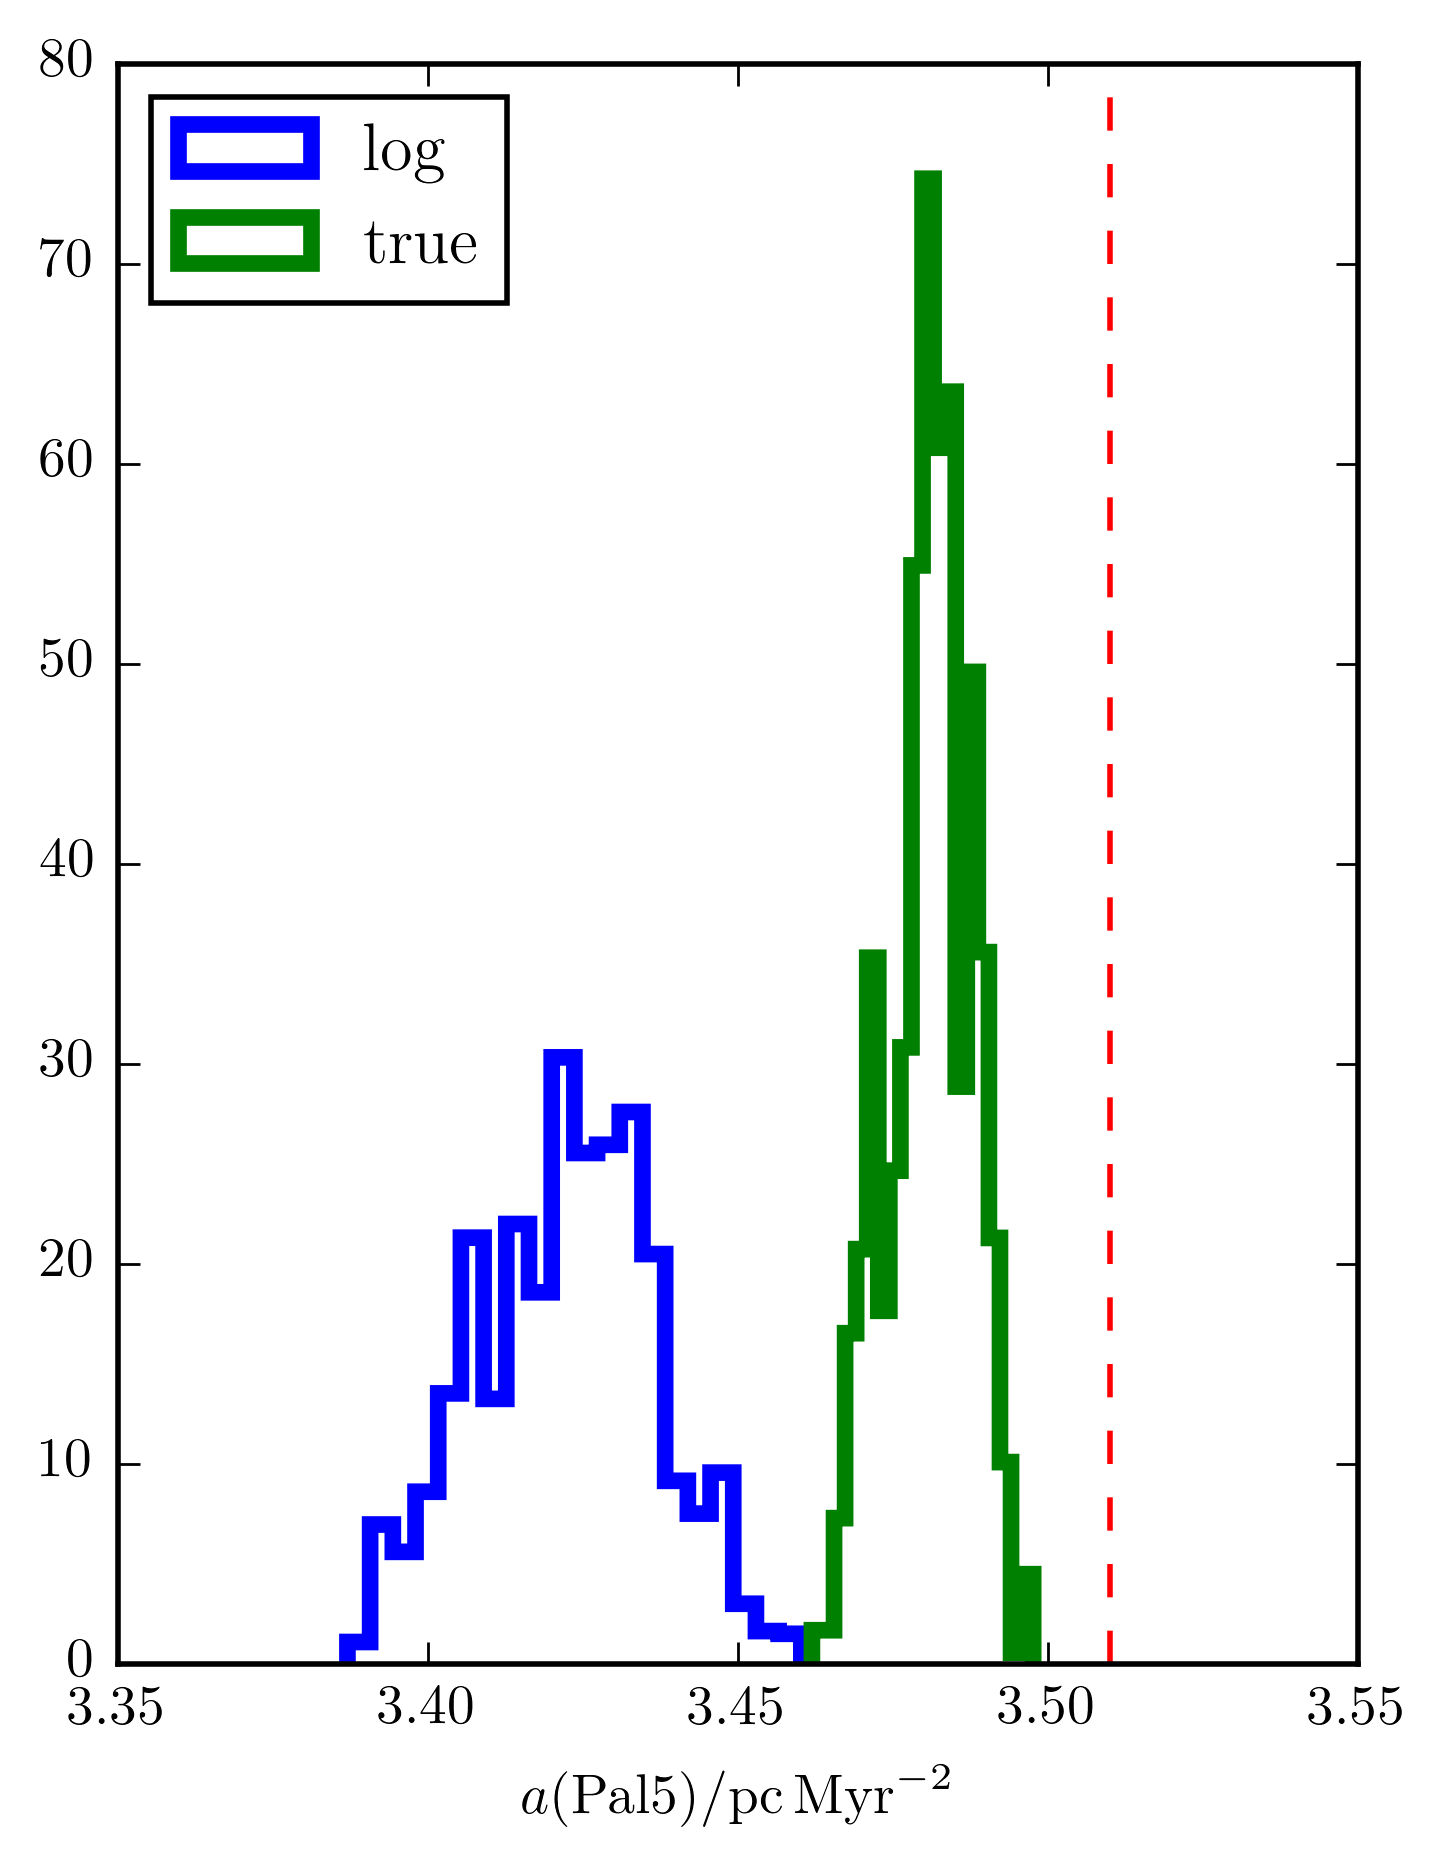
\includegraphics[width=83mm]{./figures/jason_acc.png}
  \caption{Jason's results (Sec.~\ref{ssec:jason_results})}
  \label{plot_jason_acc}
\end{figure}

The blue histogram in Fig.~\ref{plot_jason_acc} is the acceleration-at-Pal5 distribution using the logarithmic and green is using the correct potential form. The red line shows the true value.
